% !TeX program = lualatex
% !TeX encoding = utf8
% !TeX spellcheck = uk_UA
% !TeX root =../ClassicalEletrodynamics.tex

%=========================================================
\chapter{Базові поняття та рівняння}\label{\currfilebase}
%=========================================================

%% --------------------------------------------------------
\section{Величини, що спостерігаються в електродинаміці}
%% --------------------------------------------------------

%% --------------------------------------------------------
\subsection*{Заряд, електричне та магнітне поле}
%% --------------------------------------------------------


Основними спостережуваними величинами в електродинаміці є
електричний заряд та електромагнітне поле --- сукупність електричного та
магнітного полів. Статичні заряди створюють електричне поле, рух зарядів
спричинює магнітне поле. Навпаки, електромагнітне поле створює силу, що діє
на заряджене тіло. Ця схема відповідає концепції близькодії, яка домінує в
сучасній фізиці; за цією концепцією заряди взаємодіють між собою через
електромагнітне поле, а не безпосередньо.

%% --------------------------------------------------------
\subsection*{Закон Кулона}
%% --------------------------------------------------------

Числову характеристику заряду можна дати, вимірюючи
силу взаємодії F між двома точковими нерухомими зарядами. Якщо ці заряди
розташовані на відстані R, за абсолютною величиною:
\begin{equation}\label{eq:Columb_low}
    F = k \frac{q_1q_2}{R^2},
\end{equation}
де $q_1$, $q_2$ --- заряди тіл, $k$ --- коефіцієнт пропорційності, що залежить від вибору
системи одиниць. Це співвідношення називають законом Кулона; воно
неодноразово перевірялося різними експериментальними методами. Сила, з
якою один заряд діє на інший, направлена вздовж лінії центрів зарядів.
З спостережень відомо, що існують лише два сорти електричних зарядів,
причому заряди однакового сорту завжди притягуються, а заряди різного сорту
— відштовхуються. Цю обставину враховуємо, вводячи знаки зарядів в
формулі~\eqref{eq:Columb_low}. Від'ємними вважаються заряди того ж сорту, що й заряд
електрона. Заряд є адитивною числовою величиною: заряд будь-якої
системи є алгебраїчною сумою зарядів його підсистем.

Формула~\eqref{eq:Columb_low} дає змогу визначити заряд й подати процедуру його
вимірювання (тобто спосіб порівняння заряду з деяким еталоном) за
допомогою вимірювання сили взаємодії. В гаусовiй системi одиниць два
одиничних заряди створюють силу взаємодiї $1\ \text{дина} = 1\ \text{г}\cdot\text{см} / \text{c}^2$,
якщо знаходяться на відстані $1$~см. Відповідно в~\eqref{eq:Columb_low} слід покласти $k=1$. Це --- означення
одиничного заряду в гаусовій системі (тут одиниця заряду не має спеціальної назви):
\begin{equation*}
    \left[q\right] = \text{г}^{1/2}\cdot\text{см}^{3/2}\cdot\text{с}^{-1}.
\end{equation*}

Підкреслимо, що в~\eqref{eq:Columb_low} йдеться про точкові сферичні заряди, тобто
такі, взаємодія яких не залежить від їх орієнтації. Справа в тому, що хоча
точкове тіло --- це таке, розмірами якого можна знехтувати, в конкретній задачі
розподіл зарядів всередині цього тіла може бути різко неоднорідним. Це
спричинюватиме, взагалі кажучи, відмінність сили взаємодії від~\eqref{eq:Columb_low}.
Прикладом може служити взаємодія точкових диполів. Далі під точковим
зарядом ми будемо розуміти саме сферичний точковий заряд, якщо немає
інших застережень.

%% --------------------------------------------------------
\subsection*{Напруженість електричного поля та індукція магнітного поля}
%% --------------------------------------------------------

 Числову характеристику електромагнітного поля можна дати,
вимірюючи сили, що діють на рухомий електричний пробний заряд. Пробний
заряд --- це такий, впливом якого на зовнішнє поле можна знехтувати.
 З експерименту відомо, що на заряджене точкове пробне тіло (сферичний
точковий заряд) в електромагнітному полі діє сила Лоренца:
\begin{equation}\label{eq:Lorentz_force}
    \vect{F} = q\left( \Efield + \frac1c \left[ \vect{v}\times\Bfield\right] \right),
\end{equation}
де $q$ --- заряд тіла що не залежить від швидкості, $\vect{v}$ --- його швидкість, а вектори $\Efield$
та $\Bfield$ не залежать від тіла і є характеристиками поля; коефіцієнт $c$ визначається системою одиниць.

Вектор $\Efield$ називають напруженістю електричного поля, $\Bfield$ --- індукцією
магнітного поля. Сукупність цих двох векторів, заданих в кожній точці
простору, повністю визначають стан електромагнітного поля в класичній
фізиці. Формула \eqref{eq:Lorentz_force} також дозволяє узагальнити процедуру визначення
заряду на випадок руху тіла. Адже спосіб, що базується на законі Кулона
\eqref{eq:Columb_low}, працює лише для нерухомих зарядів.
Спостерігаючи за рухом заряджених частинок, можна визначити (див. вправу \ref{prb:1}) напруженість електричного поля та індукцію магнітного поля.
Звичайно, на практиці існують більш зручні методи вимірювання $\Efield$ та $\Bfield$.

%=========================================================
\begin{problem}\label{prb:1}%
Нехай в експерименті визначають прискорення в однорідному
електромагнітному полі електронів з заданими початковими швидкостями.
Покажіть, що це дає змогу однозначно визначити вектори $\Efield$
та $\Bfield$ за формулою~\eqref{eq:Lorentz_force}.
\end{problem}

В гаусовій системі одиниць коефіцієнт $с = 2,9979⋅1010$~см/с --- швидкість
світла, тому розмірності $\Efield$
та $\Bfield$ формально однакові:
\begin{equation*}
    \left[ E\right]  = \left[ B \right]  = \text{г}^{1/2}\cdot\text{см}^{-1/2}\cdot\text{с}^{-1}.
\end{equation*}
Одиниця магнітної індукції має назву <<Гаусс>>. Її не застосовують у випадку
електричного поля, хоча формально його напруженість має цю ж розмірність.


%% --------------------------------------------------------
\subsection*{Основні властивості зарядів та електромагнітного поля}
%% --------------------------------------------------------

\begin{itemize}
\item Принцип суперпозиції.

Формула~\eqref{eq:Lorentz_force} дає змогу виміряти
електромагнітне поле, вивчаючи його вплив на рух точкового заряду, але не
дозволяє його розрахувати, виходячи з розподілу зарядів. Для цього потрібні

рівняння, що пов’язують певним чином електромагнітне поле з його
джерелами. Але перш ніж записати ці рівняння, відзначимо фундаментальний
принцип суперпозиції електромагнітних полів: напруженість електричного
поля $\Efield$ та індукція $\Bfield$ магнітного поля, створюваних системою зарядів, є сумою
полів $\Efield_k$ , $\Bfield_k$, що створюються окремими зарядами (або підсистемами) цієї
системи:
\begin{equation}
    \Efield = \sum\limits_k \Efield_k, \quad \Bfield = \sum\limits_k \Bfield_k.
\end{equation}
 Тут поле $(\Efield_k, \Bfield_k)$ $k$-ї підсистеми розглядається окремо.
 Це твердження, яке значно спрощує розв’язання задач електродинаміки,
випливає з дослідних даних. Взагалі кажучи, можна навести приклади, коли
фізичні поля не задовольняють принципу суперпозиції. Але ці явища класична
електродинаміка не розглядає. В звичайних умовах принцип суперпозиції
виконується з дуже високою точністю. Принцип суперпозиції тісно пов’язаний
з адитивністю заряду.


\item Квантування (дискретність) електричного заряду.


З експериментів відомо, що найменшим відомим зарядом є заряд електрона, що наближено дорівнює (за абсолютною величиною) $е=4,8\cdot10^{-10}$ одиниць
гаусової системи. Заряд електрона є від’ємним; заряд протона – додатній і дорівнює заряду електрона з оберненим знаком. Будь-які заряди, що
спостерігалися, кратні заряду електрона. Пошуки вільних зарядів, менших за е, або не кратних цій величині, дали негативний результат. Зауважимо, що
відхилення зарядів протона й електрона призвело б до порушення електронейтральності атомів, що суперечить експериментальним даним. Слід відзначити, що
сучасні експерименти дають змогу вивчати розподіл заряду всередині елементарних часток. Але наявність неперервного розподілу густини заряду всередині,
наприклад, протона чи нейтрона, яка досліджується при зіткненнях елементарних часток, не суперечить квантуванню електричного заряду. Ця властивість
стосується повного заряду частинок, що можуть існувати iзoльовано від інших.


\item Інваріантність електричного заряду.


Величина заряду не залежить від
його швидкості відносно спостерігача. Неінваріантність заряду також могла б
призвести до порушення електронейтральності атомів, оскільки електрони в
атомах рухаються з швидкостями до 0,1 с; величина швидкості електронів
різна на різних оболонках і відрізняється в різних атомах.



\item Збереження електричного заряду.



Якщо вважати встановленим факт
квантування заряду, то збереження заряду в звичайних умовах пов’язано зі
збереженням кількості протонів та електронів в атомах. Однак відомо, що
електричний заряд зберігається і тоді, коли мають місце взаємоперетворення
елементарних часток.

Область застосовності законів збереження, квантування та інваріантності
електричного заряду виходить далеко за рамки класичної електродинаміки. На
цей час порушення цих законів невідомі.

\end{itemize}

%% --------------------------------------------------------
\subsection*{Розподіли зарядів та струмів}
%% --------------------------------------------------------

\begin{itemize}

%% --------------------------------------------------------
\item Сила струму.
%% --------------------------------------------------------


Дамо числову характеристику електричного струму --- впорядкованого руху носіїв заряду.
Нехай поверхня $S$ є орієнтованою, тобто визначений певний додатній
напрямок перетину цієї поверхні. Нехай $q(t)$ --- сумарний заряд, що перетнув $S$ з
урахуванням напрямку за час t з початку відліку. Тоді, за визначенням, сила
струму через поверхню $S$ (в додатному напрямку) є:
\begin{equation}\label{eq:I_S}
    I_S(t) = \frac{dq(t)}{dt}.
\end{equation}

У разі сталого струму --- це заряд, що перетинає $S$ за одиницю часу.


\begin{itemize}
\item  Здавалося б, що запис \eqref{eq:I_S} не є цілком коректний, оскільки заряди дискретні і $q(t)$ змінюється стрибками. Однак завдяки малості цих
стрибків $q(t)$ можна апроксимувати гладкою функцією, що є цілком правомірно в макроскопічних застосуваннях.
\item  Необхідними елементами визначення сили струму є поверхня $S$ та її орієнтація. Але якщо йдеться про сталий струм в провідникові, форма перерізу,
через який обчислюється струм, не є суттєвою. Завдяки закону збереження заряду струм через $S_1$, $S_2$ та $S_3$ (див. рис.~\ref{tikz:current})
однаковий. Адже у
разі супротивного заряд з часом міг би накопичуватися, наприклад, між $S_1$ та $S_2$, що суперечило б умові стаціонарності.
\end{itemize}

%---------------------------------------------------------
\begin{SCfigure}[1][h!]
    \centering
    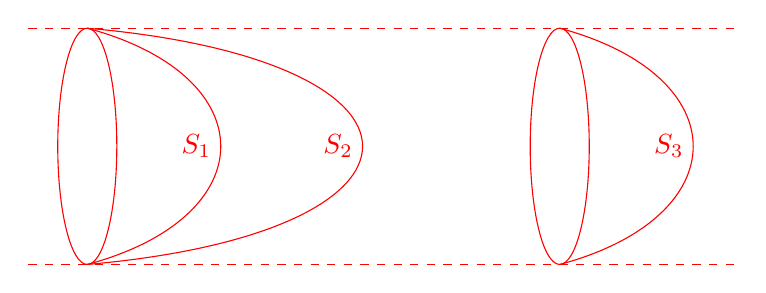
\begin{tikzpicture}[scale=1.5]
        \def\R{1}
        \draw[red, dashed] (0, {+\R}) -- ++(6, 0);
        \draw[red, dashed] (0, {-\R}) -- ++(6, 0);
        \draw[red] (0.5, 0) circle (0.25 and \R);
        \draw[red] (0.5, {+\R}) to[out=-15, in=15, looseness=2] node[pos=0.5, left] {$S_1$} (0.5, {-\R}) ;
        \draw[red] (0.5, {+\R}) to[out=-5, in=5, looseness=4] node[pos=0.5, left] {$S_2$} (0.5, {-\R}) ;

        \draw[red] (4.5, 0) circle (0.25 and \R);
        \draw[red] (4.5, {+\R}) to[out=-15, in=15, looseness=2] node[pos=0.5, left] {$S_3$} (4.5, {-\R}) ;
    \end{tikzpicture}
\caption{}
\label{tikz:current}
\end{SCfigure}
%---------------------------------------------------------


%% --------------------------------------------------------
\item Мікроскопічний та макроскопічний підхід в електродинаміці.
%% --------------------------------------------------------



Мікроскопічний підхід оперує з якомога точними значеннями величин, що характеризують електромагнітні взаємодії з врахуванням будови речовини і в цьому
розумінні він є найбільш повним та послідовним. Але використання мікроскопічного підходу не завжди доцільно. Приклад такої ситуації – попереднє
обговорення формули~\eqref{eq:I_S}). У макроскопічних вимірюваннях амперметр вимірює усереднене значення сили струму, і тут можна не зважати на
дискретну будову електрики. Це дає змогу застосовувати відповідну математичну модель процесу вимірювання, яка працює з гладкими функціями $I_S(t)$ та
$q(t)$ в~\eqref{eq:I_S}). Якщо треба охарактеризувати нерівномірність розподілу зарядів в об’ємі, можна також використовувати ідеалізацію, коли
вводиться густина заряду, яка є неперервною функцією координат. Це можливо, якщо кожна ділянка цього об’єму, де виконують вимірювання, містить досить
велику кількість елементарних зарядів. Далі під макроскопічними величинами будемо розуміти такі, що отримані внаслідок деякого усереднення --- за часом
або у деяких просторових масштабах. З одного боку макроскопічний підхід пов’язаний з можливостями конкретного фізичного експерименту, в якому
мікробудова може бути несуттєвою, з іншого боку, застосування неперервних розподілів дає змогу застосувати апарат математичного аналізу для опису явищ.



%% --------------------------------------------------------
\item  Густина заряду.
%% --------------------------------------------------------


Для опису заданого просторового розподілу заряду
введемо функцію ρ, що може залежати від координат та від часу і дозволяє
обчислити заряд в будь-якій області $\Omega$ за формулою:
\begin{equation}\label{eq:q}
    q_{\Omega} = \iiint\limits_{\Omega} \rho(t, \vect{r}) dV
\end{equation}
де $\vect{r} = x\vect{e}_x + y\vect{e}_y + z\vect{e}_z$, $dV=dx\ dy\ dz$.

Інакше, елемент заряду в об’ємі $dV$ --- це є $dq = \rho(t, \vect{r}) dV$.

Функцію $\rho(t, \vect{r})$ називають густиною заряду. Для сталого розподілу це є
величина заряду в одиниці об’єму.

Якщо в середовищі присутні однакові носії з зарядом $q$ й об’ємною
густиною їх числа (концентрацією) $n$:
\begin{equation}
    \rho = qn
\end{equation}
а в більш загальному випадку:
\begin{equation}
    \rho(t, \vect{r}) = \sum\limits_k q_kn_k(t, \vect{r}),
\end{equation}
де індекс $k$ відповідає різним сортам носіїв заряду, кожен із своєю концентрацією.


%% --------------------------------------------------------
\item Густина струму.
%% --------------------------------------------------------


Цю величину можна визначити формулою для сили
струму через поверхню $S$:
\begin{equation}
    I_S(t) = \iint\limits_S \vect{j}(t, \vect{r})\cdot d\vect{S},
\end{equation}
де $\vect{j}$ --- вектор густини струму, що не залежить від $S$, $d\vect{S} = \vect{n} dS$, $\vect{n}$ --- нормаль до
елемента поверхні $dS$. Густина сили струму дає напрям руху зарядів в даному
елементі об’єму і за абсолютною величиною --- силу струму через одиничний
переріз, проведений перпендикулярно до цього напрямку. Маємо:
\begin{equation}
    \vect{j} = nq\vect{v}
\end{equation}
якщо усі заряди з концентрацією $n$ мають однакову швидкість $\vect{v}$ та заряд $q$,
або для декількох сортів носіїв заряду:
\begin{equation}
\vect{j} = \sum\limits_k q_k n_k\vect{v}_k
\end{equation}
Ще більш загальний вираз можна записати за наявності розподілу за
швидкостями:
\begin{equation}
\vect{j} = \sum\limits_k \int  q_k f_k(t, \vect{r}, \vect{v}) \vect{v}_k dV_xdV_ydV_z,
\end{equation}
де $f_k(t, \vect{r}, \vect{v})$ --- функція розподілу k–го сорту зарядів за швидкостями.


%% --------------------------------------------------------
\item Поверхневі заряди та струми.
%% --------------------------------------------------------


 Якщо електричні заряди зосереджені у
тонкому прошарку поблизу деякої поверхні, доцільно ввести поверхневу
густину заряду σ. Аналогічно \eqref{eq:q}, покладемо:
\begin{equation}
    q_S(t) = \iint\limits_S \sigma(t, \xi, \eta) dS(\xi, \eta).
\end{equation}
де $q_S$ --- заряд на ділянці S цієї поверхні, $\xi$ та $\eta$ --- координати на поверхні; $\sigma$
характеризує вміст заряду на одиниці площі.


%---------------------------------------------------------
\begin{SCfigure}[2][h!]
    \centering
    \begin{tikzpicture}[scale=1.5]
        \draw[midarrow, tangent=0.2, tangent=0.4, tangent=0.6, tangent=0.8, red, thick] (-1, 1) node[above, text=red] {$L$} to[out=-90, in=115] (0, -1) ;
        \foreach \i in {1,...,4}{
            \draw[->, use tangent=\i, blue] (0,0) coordinate (T\i)-- ++(90:0.5);
            \draw[->] (T\i) -- ++(1, 0);
            \draw[] (T\i) -- ++(-1, 0);
        }
    \end{tikzpicture}
\caption{}
\label{surface_current}
\end{SCfigure}
%---------------------------------------------------------

 За наявності руху поверхневих зарядів визначимо силу струму через лінію
$L$ (див. рис.~\ref{surface_current}) на цій поверхні:
\begin{equation}
    I_L(t) = \frac{dq_L(t)}{dt},
\end{equation}
де $dq_L$ --- заряд, що перетинає $L$ за час $ t$ з початку спостереження. Тут також
має бути зафіксований додатній напрямок при перетині L вздовж цієї поверхні.
Лінійна густина i поверхневого струму визначається формулою (для будьякої лінії $L$ на поверхні):
\begin{equation}
    I_L(t) = \int\limits_L \vect{i}(t, \xi, \eta) d\vect{l}(\xi, \eta),
\end{equation}
де $d\vect{l} = \vect{n} d \ell$ --- орієнтовний елемент довжини на $L$, $\vect{n}$ --- нормаль до $L$ на поверхні у
точці інтегрування.

\end{itemize}

%% --------------------------------------------------------
\subsection*{Математичний запис закону збереження заряду}
%% --------------------------------------------------------


Нехай $q_{\Omega}$ --- заряд в деякому об'ємi $\Omega$, $\partial\Omega$ --- поверхня, що обмежує цей
об'єм, $I_{\partial\Omega}$ --- струм, що виходить через $\partial\Omega$ назовні з об'єму $\Omega$ (будемо вважати,
що це відповідає додатній орiєнтацiї поверхнi $\Omega$). Тоді, за законом збереження заряду i за означенням струму~\eqref{eq:I_S}, маємо у кожний момент
часу:
\begin{equation}\label{eq:charge_conservation_low_int}
    \frac{dq_{\Omega}}{dt} + I_{\partial\Omega}   = 0.
\end{equation}

Спiввiдношення \eqref{eq:charge_conservation_low_int} є інтегральною формою закону збереження
заряду. Для поверхневих зарядів та струмів можна подати аналогічне
співвідношення, що пов’язує швидкість зміни заряду на дiлянку поверхнi та
струм через межу цiєї дiлянки.

Отримаємо з \eqref{eq:charge_conservation_low_int} диференціальне спiввiдношення для густини заряду
$\rho(t, \vect{r})$ та густини об'ємного струму $\vect{j}(t, \vect{r})$ . Використовуючи визначення \eqref{eq:q}
для нерухомого об'єму:
\begin{equation*}
    \frac{dq_{\Omega}}{dt} = \frac{d}{dt} \iiint\limits_{\Omega} \rho(t, \vect{r}) dV = \iiint\limits_{\Omega} \frac{\partial\rho(t, \vect{r})}{\partial
    t} dV.
\end{equation*}

Тодi з \eqref{eq:charge_conservation_low_int}  та за виначенням густини струму \eqref{eq:I_S}:
\begin{equation*}
    \iiint\limits_{\Omega} \frac{\partial\rho(t, \vect{r})}{\partial
    t} dV + \iint\limits_{\partial\Omega} \vect{j}\cdot d\vect{S} = 0.
\end{equation*}
Перетворимо iнтеграл по замкненiй поверхнi $\partial\Omega$, що оточує об'єм $\Omega$, за
теоремою Остроградського-Гаусcа:
\begin{equation*}
    \iint\limits_{\partial\Omega} \vect{j}\cdot d\vect{S} = \iiint\limits_{\Omega}\Div\vect{j} dV,
\end{equation*}
звідки
\begin{equation*}
    \iiint\limits_{\Omega} \left(\frac{\partial\rho(t, \vect{r})}{\partial
    t}  +  \Div\vect{j} \right) dV =0.
\end{equation*}

Це співвідношення виконується для будь-якого об'єму $\Omega$, тому
підінтегральний вираз має дорівнювати нулю:
\begin{equation}\label{eq:charge_conservation_low_diff}
    \frac{\partial\rho(t, \vect{r})}{\partial t}  +  \Div\vect{j}  = 0
\end{equation}

Це диференцiальна форма закону збереження заряду або рівняння неперервності для об’ємної густини зарядів.


%% --------------------------------------------------------
\section{Рівняння електромагнітного поля}
%% --------------------------------------------------------


%% --------------------------------------------------------
\subsection*{Мікроскопічні рівняння Максвелла (інтегральна форма)}
%% --------------------------------------------------------


В цьому розділі буде розглянута система рівнянь, яка дає змогу аналізувати електродинамічні явища в усій класичній області від мікроскопічних до
макроскопічних масштабів. В рамках класичної електродинаміки ці рівняння вважаються точними, вони не містять наближень і явно враховують усі заряди і
струми в рамках конкретного явища або теоретичної моделі. Далі будемо називати ці рівняння мікроскопічними --- на відміну від макроскопічних рівнянь,
які
припускають певні наближення або макроскопічні усереднення, наприклад, для опису поляризаційних зарядів і струмів намагнічення, що виникають у
суцільному середовищі. Мікроскопічні рівняння отримано дослідним шляхом за допомогою узагальнення великої кількості експериментальних даних. Вихідною
для нас буде інтегральна форма рівнянь Максвелла, з якої далі будуть отримані граничні умови і диференціальна форма цих рівнянь. Інтегральна форма
мікроскопічних рівнянь має вид:

\begin{align}
	\oiint\limits_{\partial\Omega} \Efield\cdot d\vect{S} & = 4\pi q_{\Omega}   \label{Int
	I},                                                                                                         \\
	\oiint\limits_{\partial\Omega} \Bfield\cdot d\vect{S} & = 0   \label{Int
	II},                                                                                                                                   \\
\end{align}
де $\Omega$ --- довільний нерухомий об'єм, $\partial\Omega$ --- його межа; $S$ --- довільна нерухома орієнтована поверхня, $\partial S$ --- замкнений
контур, що її обмежує, $q_{\Omega}$ --- повний заряд в області $\Omega$.

\begin{align}
	\oint\limits_{\partial S} \Efield\cdot d\vect{r}  & = - \frac1c \iint\limits_S \frac{\partial\Bfield}{\partial t}\cdot d\vect{S}  \label{Int
	III},                                                          \\
	\oint\limits_{\partial S} \Bfield\cdot d\vect{r}  & =\dfrac{4\pi}{c} I_S +\frac{1}{c} \iint\limits_S
	\frac{\partial\Efield}{\partial t}\cdot d\vect{S}  \label{Int IV},
\end{align}
де $S$ --- довільна нерухома орієнтована поверхня, $\partial S$ --- замкнений
контур, що її обмежує. $I_S$ --- струм через $S$ у додатному напрямку.

В літературі можна зустріти форму рівнянь електродинаміки для об′ємів та поверхонь, що деформуються із часом. Зокрема, замість рівняння \eqref{Int III}
часто використовують зв’язок між електрорушійною силою, що виникає у рухомому провідникові, та зміною потоку магнітного поля через поверхню, що обмежена
контуром цього провідника. Цей зв’язок можна отримати з записаних рівнянь, якщо при обчисленні е.р.с. врахувати також внесок сил, що діють на носії
струму з боку магнітного поля.


%% --------------------------------------------------------
\subsection*{Сумісність рівнянь Максвелла із законом збереження заряду}
%% --------------------------------------------------------


Наявність довільного об′єму $\Omega$ та довільної поверхні $S$ в рівняннях Максвелла є дещо незвичайним; принаймні,
треба перевірити, чи не призводить це до неоднозначностей. Наприклад, в рівнянні \eqref{Int IV} ми можемо вибрати різні поверхні $S_1$ і
$S_2$, що мають спільну межу $\partial S$ (рис.~\ref{tikz:surface}).
%---------------------------------------------------------
\begin{SCfigure}[][h!]
	\centering
\begin{tikzpicture}[>=latex]

    \coordinate (O) at (-0.25, 0);

	\fill[thick, red, rotate around={-15:(O)}, red!50] (O) circle(1 and 0.3);

    \node (S1) at (-1, -0.5)  {$S_1$};
    \draw[->] (S1.east) to[out=0, in=-90] (O);
    \draw[thick, red, rotate around={-15:(O)}, dashed] (O) ++(180:-1) arc(0:180:1 and 0.3);
    \draw[thick, ->, rotate around={-15:(O)}, fill=red!50] (O) -- ++(0, 0.5);
	\draw[red!50, fill=red!50, rotate around={-15:(O)}, tangent=0.45, opacity=0.5] ($(O)-(1,0)$) to[out=80, in=40, looseness=4.8]
	coordinate[pos=0.2] 	(s2) 	(0.75, 0) arc(0:-180:1 and 0.3) -- cycle;

     \draw[thick, rotate around={-15:(O)}, use tangent=1, ->] (0,0) -- ++(90:0.5);

    \draw[thick, red, rotate around={-15:(O)}] (O) ++(180:1) arc(180:360:1 and 0.3);
%		\draw[fill=red!50, opacity=0.5] (0, -1.5) circle[x radius=1 cm, y radius= 0.3 cm];
%        \draw[->] (0, -1.5) -- ++(0, 1) node[left] {$n$};
%		\draw[in=55, out=125, looseness=3.9, fill=red!50, opacity=0.75] (-1, -1.5) to (+1, -1.5) arc[x radius=1 cm, y radius= 0.3 cm, start
%				angle=0,
%				delta angle=180] --cycle;
%
%        \draw[->] (0, 0.5) -- ++(0, 1) node[left] {$n$};


    \node (S2) at (-1, +2)  {$S_2$};
    \draw[->] (S2.east) to[out=0, in=90] (s2);

    \end{tikzpicture}
\caption{}
\label{tikz:surface}
\end{SCfigure}
%---------------------------------------------------------

Тоді з рівняння \eqref{Int IV} легко отримати:
\begin{equation}\label{eq:diff4}
    \frac{4\pi}c(I_{S_1} - I_{S_2}) +\frac1c \left( \iint\limits_{S_1}
	\frac{\partial\Efield}{\partial t}\cdot d\vect{S}  - \iint\limits_{S_2}
	\frac{\partial\Efield}{\partial t}\cdot d\vect{S}  \right) = 0
\end{equation}
Чи суперечить це іншим рівнянням? Виявляється, ні, якщо врахувати закон збереження заряду. Нехай $\Omega$ --- це область, оточена поверхнями $S_1$ та
$S_2$. Межа $\partial\Omega$ має орієнтацію, спільну з однією з цих поверхонь і протилежну до іншої на відповідних ділянках. Тоді рівняння
\eqref{eq:diff4} можна переписати так:
\begin{equation}
    4\pi I_{\partial\Omega} + \frac{d}{dt} \iint\limits_{\partial\Omega} \Efield\cdot d\vect{S} = 0,
\end{equation}
де похідну винесено за знак інтегралу. Оскільки поверхневий інтеграл тут в силу \eqref{Int I} пов’язаний із зарядом $q_{\Omega}$ в області $\Omega$,
звідси:
\begin{equation}\label{eq:charge_conservation_low}
    I_{\partial\Omega} + \frac{q_{\Omega}}{dt} = 0.
\end{equation}

Таким чином, рівняння \eqref{eq:diff4} тотожно виконується внаслідок рівняння
\eqref{Int I} та закону збереження заряду \eqref{eq:charge_conservation_low}.
У разі рівняння \eqref{Int III} ми можемо також вибрати різні поверхні
інтегрування з однаковою межею; тут аналогічні міркування з огляду на
рівняння \eqref{Int II} також показують відсутність суперечностей.


%% --------------------------------------------------------
\subsection*{Диференціальна форма рівнянь Максвелла}
%% --------------------------------------------------------


В рівнянні \eqref{Int I} за означенням:
\begin{equation}
    q_{\Omega} = \iiint\limits_{\Omega} \rho dV
\end{equation}
де $\rho$ ---  об′ємна густина заряду. За теоремою Остроградського-Гаусса ліва частина \eqref{Int I} також зводиться до об′ємного інтегралу, звідки:
\begin{equation*}
     \iiint\limits_{\Omega} \Div\Efield dV = \iiint\limits_{\Omega} \rho dV
\end{equation*}
зважаючи на довільність області $\Omega$:
\begin{equation}\label{eq:M1D}
    \Div\Efield = 4\pi\rho
\end{equation}
Аналогічно, з \eqref{Int II} маємо:
\begin{equation}\label{eq:M2D}
    \Div\Bfield = 0.
\end{equation}
В рівнянні \eqref{Int III} перетворимо ліву частину за теоремою Стокса:
\begin{equation*}
    \iint\limits_{S} \Rot\Efield\cdot d\vect{S} = - \frac1c \iint\limits_S \frac{\partial\Bfield}{\partial t}\cdot d\vect{S}
\end{equation*}
звідки, з урахуванням довільності $S$:
\begin{equation}\label{eq:M3D}
    \Rot\Efield = - \frac1c \frac{\partial\Bfield}{\partial t}.
\end{equation}
Аналогічно, виражаючи також згідно до \eqref{eq:charge_conservation_low} струм у правій частині
eqref{Int IV}  через інтеграл від густини струму $\vect{j}$, отримаємо:
\begin{equation}\label{eq:M4D}
    \Rot\Bfield = \frac{4\pi}c\vect{j} + \frac1c \frac{\partial\Efield}{\partial t}.
\end{equation}
Рівняння \eqref{eq:M1D} -- \eqref{eq:M4D} складають систему мікроскопічних рівнянь
Максвелла у диференціальній формі.

З рівнянь Максвелла \eqref{eq:M1D}, \eqref{eq:M4D} можна виразити густини заряду та
струму через напруженості полів. Виникає питання, чи не суперечитимуть ці
рівняння закону збереження заряду \eqref{eq:charge_conservation_low}, де цих напруженостей немає. Це
питання вище було розглянуто на основі інтегральної форми рівнянь
Максвелла. Покажемо це також за допомогою диференціальної форми рівнянь.
Візьмемо дивергенцію від обох частин \eqref{eq:charge_conservation_low} враховуючи, що $\Div\Rot\equiv0$:
\begin{equation*}
    0 = \frac{4\pi}c\Div\vect{j} + \frac1c \frac{\partial}{\partial t} \Div\Efield.
\end{equation*}
Підставляючи $\Div\Efield$ з \eqref{eq:M1D} отримаємо:
\begin{equation*}
    \Div\vect{j} + \frac{\partial\rho}{\partial t} = 0.
\end{equation*}
що збігається з рівнянням неперервності \eqref{eq:charge_conservation_low} --- диференціальною формою
закону збереження заряду.
Зауважимо, що обчислення дивергенції від обох частин \eqref{eq:M3D} з
урахуванням \eqref{eq:M2D} приводить до тотожності.


%% --------------------------------------------------------
\subsection*{Умови на поверхні розриву}
%% --------------------------------------------------------


Досить часто трапляється ситуація, коли поля $\Efield$ або $\Bfield$ мають розриви
першого роду на деякій поверхні $S$, залишаючись скінченними і неперервними
при переміщеннях вздовж цієї поверхні. Це пов′язано з існуванням
поверхневих зарядів та струмів на $S$ з густинами $\sigma$ та $\vect{i}$ відповідно.

Для отримання граничних умов на поверхні розриву, розглянемо довільний
досить малий елемент поверхні $S$, котрий можна вважати майже плоским.

Нехай $\vect{n}$ --- нормаль до площини розриву, що розділяє $1$ та $2$, причому
$\vect{n}$ напрямлена з $1$ в $2$

\begin{SCfigure}[0.5][h!]
	\centering
	\localinput{bc1.tikz}
	\caption{До виведення першої граничної умови}%
	\label{tikz:bc1}
\end{SCfigure}

Нехай $\Omega$ --- область всередині циліндра
(рис.~\ref{tikz:bc1}), з основами $S_1$ та $S_2$,
паралельними $S$, причому $S_1$ лежить у
середовищі $1$, $S_2$ --- в $2$, а висота циліндра дорівнює $h$.

Застосуємо рівняння \eqref{Int I} розбиваючи інтеграл по $\partial\Omega$ на частини, що відповідають $S_1$, $S_2$ та боковій поверхні
циліндра $\partial\Omega'$:
\begin{equation*}
    	\iint\limits_{S_1} \Efield\cdot d\vect{S} +  \iint\limits_{S_2} \Efield\cdot d\vect{S} + \iint\limits_{\partial\Omega'} \Efield\cdot
    	d\vect{S} = 4\pi q_{\Omega},
\end{equation*}
де повний заряд всередині $\Omega$ складається в загальному випадку з неперервнорозподіленого об′ємного заряду iз інтегрованою об’ємною
густиною ρ та поверхневого заряду з поверхневою густиною $\sigma$ на $S$:
\begin{equation*}
    q_{\Omega} = \iiint\limits_{\Omega} \rho dV + \iint\limits_S \sigma dS.
\end{equation*}


Якщо висота $h  \to 0$, об'єм та бокова поверхня циліндра також прямують до нуля, а з ними й інтеграли по об′єму та по бічній поверхні. Відкидаючи ці
інтеграли, отримаємо:
\begin{equation*}
    	\iint\limits_{S_1} \Efield_1\cdot d\vect{S} +  \iint\limits_{S_2} \Efield_2\cdot d\vect{S}  = 4\pi q_{\Omega}.
\end{equation*}
Оскільки:
\begin{equation*}
    \iint\limits_{S_1} \Efield_1\cdot d\vect{S}  = - \iint\limits_{S} \Efield_1\cdot \vect{n}\ dS, \quad \\
    \iint\limits_{S_2} \Efield_2\cdot d\vect{S} = \iint\limits_{S} \Efield_1\cdot \vect{n}\ dS,
\end{equation*}
де враховано напрямки нормалей до $\partial\Omega$ на $S_1$ та $S_2$, звідки:
\begin{equation*}
    \iint\limits_{S} (\Efield_2 - \Efield_1)\cdot\vect{n}\ dS = 4\pi \iint\limits_S \sigma dS.
\end{equation*}
Завдяки довільності $S$, дістаємо співвідношення в будь-якій точці поверхні
розриву:
\begin{equation}\label{eq:bc1}
    (\Efield_2 - \Efield_1)\cdot\vect{n} = 4\pi\sigma,
\end{equation}
яке пов’язує нормальні до поверхні розриву складові напруженості
електричного поля з обох боків розриву.

\begin{SCfigure}[0.5][h!]
	\centering
	\localinput{bc2.tikz}
	\caption{До виведення другої граничної умови}%
	\label{tikz:bc2}
\end{SCfigure}

Щоб отримати зв’язок тангенціальних компонент E, звернемося до рівняння \eqref{Int III}. Розглянемо прямокутний контур, дві сторони $BC$ і $AD$
(рис.~\ref{tikz:bc2}) якого паралельні до поверхні розриву.

З рівняння \eqref{Int III}:
\begin{equation*}
    \int\limits_{AB} \Efield\cdot d\vect{r} + \int\limits_{BC} \Efield\cdot d\vect{r} + \int\limits_{CD} \Efield\cdot d\vect{r} + \int\limits_{DA}
    \Efield\cdot d\vect{r} =
    -\frac1c \frac{\partial\Bfield}{\partial t}\cdot d\vect{S}.
\end{equation*}
Інтеграл по $S$ (за умови неперервності $\frac{\partial\Bfield}{\partial t}$) прямує до нуля при $h\to0$.
Тому, враховуючи напрямок обходу контура, що визначає знак інтегралів по
$BC$ і $AD$, можна записати:
\begin{equation*}
\int\limits_{BC} (\Efield_2 - \Efield_1)\cdot\vect{\tau} d\ell = 0
\end{equation*}
де $\vect{\tau}$ --- тангенціальний одиничний вектор вздовж $BC$. Звідси, завдяки
довільності вибору контура $ABCD$,
\begin{equation}\label{eq:bc2}
    (\Efield_2 - \Efield_1)\cdot\vect{\tau} = 0
\end{equation}
Очевидно, це співвідношення справедливе, якщо $\vect{\tau}$ --- довільний тангенціальний до поверхні $S$ одиничний вектор.
Легко перевірити, розглядаючи \eqref{eq:bc2} для двох незалежних напрямків $\vect{\tau}$ на
поверхні $S$, що еквівалентна формі граничних умов для тангенціальних
складових може бути записана так:
\begin{equation*}
    \left[ \vect{n}\times (\Efield_2 - \Efield_1)\right] = 0
\end{equation*}
Таким чином, тангенціальна складова напруженості електричного поля не
має розривy на $S$.

З рівняння Максвелла \eqref{Int II} отримуємо співвідношення для нормальних
компонент індукції магнітного поля аналогічно \eqref{eq:bc1}:
\begin{equation}
     (\Bfield_2 - \Bfield_1)\cdot\vect{n} = 0
\end{equation}
тобто нормальна компонента індукції магнітного поля не має розривів. Це є
наслідком відсутності магнітних зарядів, в даному випадку, поверхневих.

На відміну від цього, тангенціальна компонента $\Bfield$ може
мати розриви за наявності поверхневого струму з поверхневою густиною~$\vect{i}$.

\begin{SCfigure}[0.5][h!]
	\centering
	\localinput{bc2m.tikz}
	\caption{До виведення другої граничної умови для $\Bfield$}%
	\label{tikz:bc2m}
\end{SCfigure}

Нехай $\vect{n}$ --- вектор нормалі до поверхні, проведений з $1$ в $2$,  $\vect{\tau}$ --- тангенціальний одиничний вектор вздовж $BC$, а $\vect{b}$
--- вектор, що перпендикулярний до $\vect{\tau}$ та $\vect{n}$ і утворює разом з ними праву трійку
Запишемо:
\begin{equation*}
    \Bfield = B_n\vect{n} + B_{\tau}\vect{\tau} + B_b\vect{b},
\end{equation*}
де напрямок одиничного вектора $\vect{b}$ відповідає напрямку $\vect{i}$, напрямок
одиничного вектора $\vect{\tau}$ перпендикулярний до $\vect{n}$ та $\vect{b}$.
З рівняння \eqref {Int IV} для контура $ABCD$ при $h \to 0$, враховуючи, що за цієї
умови інтеграли по сторонам $AB$ і $CD$ прямують до нуля, маємо:
\begin{equation*}
    \int\limits_{BC} \Bfield\cdot d\vect{r} + \int\limits_{DA} \Bfield\cdot d\vect{r} = \int\limits_{BC} (\Bfield_2 - \Bfield_1)\cdot\vect{\tau} d\ell =
    \frac{4\pi}c I_{BC},
\end{equation*}
де $I_{BC} = \int\limits_{BC} \vect{i}\cdot\vect{b}\ d\ell$ --- поверхневий струм через BC. Звідси:
\begin{equation}\label{eq:bc2m}
    (\Bfield_2 - \Bfield_1)\cdot\vect{\tau} = \frac{4\pi}c\ \vect{i}\cdot\vect{b}.
\end{equation}
Розглядаючи \eqref{eq:bc2m} для двох незалежних напрямків $\vect{\tau}$ можемо написати:
\begin{equation}\label{eq:bc2m2}
    \left[ \vect{n}\times(\Bfield_2 - \Bfield_1)\right]  = \frac{4\pi}c\ \vect{i}.
\end{equation}



%% --------------------------------------------------------
\section{Закони збереження}
%% --------------------------------------------------------




%% --------------------------------------------------------
\subsection*{Збереження енергії електромагнітного поля}
%% --------------------------------------------------------


В електромагнітному полі на заряди діє сила Лоренца~\eqref{eq:Lorentz_force}. Потужність,
що витрачає ця сила, є:
\begin{equation*}
    \vect{F}\cdot\vect{v} = q\Efield\cdot\vect{v}.
\end{equation*}

Якщо концентрація зарядів є $n$, маємо $\vect{j} = qn\vect{v}$; тоді потужність, що
витрачає електричне поле в одиничному об’ємі, є:
\begin{equation}
    \frac{dA}{dt} = \vect{j}\cdot\Efield.
\end{equation}
Легко перевірити, що ця формула зберігається у разі загального розподілу
різних зарядів за швидкостями.

З рівняння \eqref{eq:M4D}:
		\begin{equation*}
			\vect{j} = \frac{c}{4\pi} \Rot\Bfield - \frac1c \parttime{\Efield}.
		\end{equation*}
звідси, за формулами векторного аналізу:
		\begin{multline*}
			\vect{j}\cdot\Efield =  \frac{c}{4\pi}\Efield\cdot\Rot\Bfield - \frac1{4\pi}\Efield\cdot\frac{\partial\Efield}{\partial t} = \\
             = - \Div\left(\frac{c}{4\pi}[\Efield\times\Bfield]\right) + \frac{c}{4\pi}  \Bfield\cdot \Rot\Efield  -
			\parttime{}
			\left( \frac1{8\pi}\Efield^2\right)
		\end{multline*}



        В силу рівняння \eqref{eq:M3D}:
		\begin{multline*}
			\vect{j}\cdot\vect{E} =  - \Div\left(\frac{c}{4\pi}[\Efield\times\Bfield]\right) - \frac{1}{4\pi}  \Bfield\cdot
			\parttime{\Bfield}  -
			\parttime{} \left( \frac1{8\pi}\Efield^2\right) = \\
             = - \Div\left(\frac{c}{4\pi}[\Efield\times\Bfield]\right) -  \parttime{} \left(
			\frac1{8\pi}\Efield^2 +
			\frac1{8\pi}\Bfield^2 \right)
		\end{multline*}

	Звідси отримуємо важливе співвідношення:
\begin{equation}\label{eq:energy_balance}
    \vect{j}\cdot\vect{E} + \Div\vect{\Pi} +  \parttime{} \frac{\Efield^2 + \Bfield^2}{8\pi}  = 0,
\end{equation}
де величину:
\begin{equation}
    \vect{\Pi} = \frac{c}{4\pi}[\Efield\times\Bfield]
\end{equation}
називають вектором Пойнтінга; як буде видно далі, він має зміст густини потоку енергії.

Співвідношення \eqref{eq:energy_balance} виражає енергетичний баланс в одиниці об’єму.
Проінтегруємо його по деякій області $\Omega$, перетворюючи інтеграл з
дивергентним членом в інтеграл по (замкненій) поверхні $\partial\Omega$, що оточує $\Omega$:
\begin{equation}\label{eq:energy_balance_int}
    \iiint\limits_{\Omega} \vect{j}\cdot\vect{E} dV + \oiint\limits_{\partial\Omega} \vect{\Pi}\cdot d\vect{S} +  \parttime{} \iiint\limits_{\Omega}
    \frac{\Efield^2 + \Bfield^2}{8\pi} dV  = 0.
\end{equation}

Перший в доданок в \eqref{eq:energy_balance_int} --- це робота, яку виконує поле за одиницю часу
в об’ємі $\Omega$, другий --- потік енергії через поверхню $\partial\Omega$, останній доданок ---
швидкість зміни енергії електромагнітного поля в об’ємі Ω. Величина:
\begin{equation}
    W = \iiint\limits_{\Omega}     \frac{\Efield^2 + \Bfield^2}{8\pi} dV
\end{equation}
являє собою енергію поля в області $\Omega$.


%% --------------------------------------------------------
\subsection*{Закон збереження імпульсу}
%% --------------------------------------------------------

Імпульс, що передає поле зарядам в одиниці об`єму, визначається силою
Лоренца~\eqref{eq:Lorentz_force}:
\begin{equation*}
    \vect{f} = \rho\Efield + \frac1c\left[\vect{j}\times\Bfield\right].
\end{equation*}

З рівняння Максвелла \eqref{eq:M1D}:
\begin{equation*}
    \rho\Efield = \frac1{4\pi}\Efield\Div\Efield,
\end{equation*}
або для $k$-ої компоненти:
\begin{equation*}
    4\pi\rho E_k = E_k\partial_iE_i = \partial_i(E_iE_k) - E_i \partial_iE_k.
\end{equation*}

Запишемо рівняння \eqref{eq:M3D} $\Rot\Efield = - \frac1c \parttime\Bfield$ покомпонентно:
\begin{equation*}
    (\Rot\Efield)_i = \epsilon_{ijk}\partial_j E_k = - \frac1c \parttime{B_i},
\end{equation*}
помножимо його на $\epsilon_{pqi}$ ε та підсумуємо по $i$:
\begin{equation*}
    \epsilon_{pqi}\epsilon_{ijk}\partial_j E_k = - \epsilon_{pqi}  \frac1c \parttime{B_i},
\end{equation*}
або, за допомогою формули згортки:
\begin{equation*}
    \partial_pE_q -  \partial_qE_p = - \epsilon_{pqi}  \frac1c \parttime{B_i}.
\end{equation*}

Враховуючи це співвідношення, дістанемо:

\begin{multline*}
     4\pi\rho E_k =  \partial_i(E_iE_k) - E_i \partial_kE_i - \frac1c \epsilon_{kij} E_i \parttime{B_j} = \\
    = \partial_i\left( E_kE_i - \frac12
     \Efield^2\delta_{ik}\right) - \frac1c \left[ \Efield \times \parttime{\Bfield}\right]_k .
\end{multline*}

З останнього рівняння Максвелла\eqref{eq:M4D} $vect{j} = \frac{c}{4\pi} \Rot\Bfield - \frac1c \parttime{\Efield}$:
\begin{multline*}
    \frac1c \left[ \vect{j}\times\Bfield\right]_k = \epsilon_{kij} j_i B_j = \frac1c  \epsilon_{kij} \left[ \frac{c}{4\pi}\epsilon_{ipq}\partial_p B_q -
    \frac1{4\pi}\parttime{E_i}
    \right] B_j = \\
    = \frac1{4\pi} \left( \delta_{kq}\delta_{jp} - \delta_{kp}\delta_{jq} \right) B_j\partial_p B_q - \frac1{4\pi c} \epsilon_{kij}\parttime{E_i} B_j =
    \\
    = \frac1{4\pi} \left( B_j \partial_j B_k - B_j \partial_k B_j \right) - \frac1{4\pi c} \left[ \parttime{\Efield}\times\Bfield\right]_k.
\end{multline*}

Це можна подати як:
\begin{equation*}
    \frac{4\pi}{c} \left[ \vect{j}\times\Bfield\right]_k = \partial_j \left( B_kB_j - \delta_{ij} \frac{\Bfield^2}{2}\right) - \frac1{4\pi c} \left[
    \parttime{\Efield}\times\Bfield\right]_k.
\end{equation*}

Маємо результат для балансу імпульсу в одиниці об'єму:
\begin{equation}
    f_k + T_{kj, j}  + \parttime{\pi_k} = 0, \quad \vect{\pi} = \frac{\vect{\Pi}}{c^2},
\end{equation}
де
\begin{equation*}
    T_{kj} = \frac1{4\pi} (E_kE_j + B_kB_j) - \frac1{8\pi}\delta_{kj}(\Efield^2 + \Bfield^2)
\end{equation*}
максвеллівський тензор натягу.

Інтегральне співвідношення:
\begin{equation}
    \iiint\limits_{\Omega} f_k dV + \oiint\limits_{\partial\Omega} T_{kj} n_j dS + \parttime{}  \iiint\limits_{\Omega} \pi_k dV = 0
\end{equation}
пов'язує зміну імпульсу в об'ємі $\Omega$ з дією зовнішніх зовнішніх сил та потоком
через бічну поверхню; тут $\pi_k$ --- імпульс поля в одиниці об'єму.


%% --------------------------------------------------------
\subsection*{Закон збереження моменту імпульсу}
%% --------------------------------------------------------


Виходимо з рівнянь:
\begin{equation*}
    \frac{d\vect{L}}{dt} = \vect{M},\quad \vect{M} = \left[\vect{r}\times\vect{f} \right].
\end{equation*}
Момент сили, що діє на заряди в одиниці об'єму, є, за означенням,
\begin{equation*}
    M_k = \epsilon_{kij}x_if_j.
\end{equation*}
Використовуючи співвідношення, отримані для баланса імпульсу, маємо:
\begin{equation*}
    \epsilon_{ijk}x_jf_k + \epsilon_{ijk}x_j T_{kj,j} + \parttime{L_i} = 0, \quad \text{де}\ L_i = \epsilon_{ijk}x_i\pi_k
\end{equation*}
можна інтерпретувати як густину момента імпульсу поля.

Завдяки симетрії $T_{kl}$ по індексах:
\begin{equation*}
    \epsilon_{ijk} x_j T_{kl, l} = \partial_l( \epsilon_{ijk}  x_jT_{kl}) -  \epsilon_{ijk}\delta_{lj}T_{kl} = \partial_l ( \epsilon_{ijk} x_j T_{kl}).
\end{equation*}

Звідси дістаємо локальне співвідношення для зміни моменту імпульсу:
\begin{equation}
    M_i + \partial_l( \epsilon_{ijk}  x_jT_{kl}) + \parttime{L_i} = 0.
\end{equation}
Рівняння баланса моменту імпульсу в об'ємі Ω має вид:
\begin{equation}
    \iiint\limits_{\Omega} M_i dV + \oiint\limits_{\partial\Omega} \epsilon_{ijk}  x_jT_{kl} n_l dS +
    \parttime{} \iiint\limits_{\Omega} L_i dV = 0.
\end{equation}



%% --------------------------------------------------------
\section{Межі застосовності класичної електродинаміки}
%% --------------------------------------------------------




%% --------------------------------------------------------
\subsection*{Квантова механіка і електродинаміка. }
%% --------------------------------------------------------


На сучасному рівні знань найбільш фундаментальним є квантовий розгляд фізичних процесів, який і визначає межі застосовності класичної теорії.
Електродинамічна система складається з заряджених частинок та електромагнітного поля; тут необхідно визначити, яка з цих складових (або уся система в
цілому) допускає класичний опис. Широке коло фізичних задач потребує квантового опису руху частинок в класичному електромагнітному полі. Основні зміни,
у порівнянні з класичною механікою, тут стосуються рівнянь~\eqref{eq:Columb_low}, \eqref{eq:Lorentz_force} та інших, пов’язаних із поняттями траєкторії,
сили, другим законом Ньютона, тощо. Перегляд цих понять у дослідженнях атомів та молекул – прерогатива квантової механіки, яка аналізує мікрооб’єкти з
розмірами $10^{-13} \div 10^{-16}$~см. Однак деякі мікропроцеси відзначають властивості твердих тіл і рідин також на макроскопічних масштабах. Хоча рух
заряджених частинок в цих задачах визначається законами квантової механіки, досить часто залишаються незмінними класичні поняття про напруженість
електричного поля та магнітну індукцію; наприклад, в рівнянні Шредінгера для електрона в атомі водню фігурує класичний кулонівський потенціал поля ядра.
Звичайно, що для визначення цих полів ми не завжди можемо прямо скористатися формулою~\eqref{eq:Lorentz_force}, що пов’язана з механікою точкової
частинки. Але зберігається класичний опис електромагнітного поля.


%% --------------------------------------------------------
\subsection*{Квантова будова випромінювання}
%% --------------------------------------------------------

За певних умов треба враховувати квантові властивості самого електромагнітного поля. Вивчення рівноважного електромагнітного випромінювання, а також
фотоелектричних явищ (М.~Планк, 1900; А.~Ейнштейн,1905) привело до висновку, що електромагнітне випромінювання має корпускулярні властивості і може
розглядатися як сукупність окремих квантів-фотонів, з енергією $Е=h\nu$, де $h$ --- стала Планка, $\nu$ --- частота випромінювання. Коли фотонів багато,
можливий класичний опис поля випромінювання. Але в слабких пучках випромінювання рахунок йде на окремі фотони і сучасна техніка дозволяє майже
поодиночну їх реєстрацію. Теоретичну базу для опису процесів, в яких суттєвими є квантові властивості і речовини, і електромагнітного поля, дає квантова
електродинаміка, яка є складовою частиною квантової теорії поля. Квантова електродинаміка передбачає суттєві зміни характеру електродинамічної взаємодії
також в області дуже сильних полів. В електричному полі з напруженістю $E \sim \frac{m_e^2 c^3}{he} = 10^{20}$~В/м необхідно враховувати процеси
народження та знищення електрон–позитронних пар. В цих умовах електромагнітне поле не може розглядатися окремо від електрон– позитронного поля, навіть
при поширенні електромагнітної хвилі в вакуумі. Складна взаємодія цих полів робить нелінійними ефективні рівняння для класичних величин $E$ та $B$;
завдяки цьому стає можливим процес розсіювання фотона фотоном. В цьому розумінні можна говорити про порушення класичного принципу суперпозиції.



%% --------------------------------------------------------
\subsection*{Електродинаміка і гравітація}
%% --------------------------------------------------------

Взаємодію гравітаційного та електромагнітного полів розглядає загальна
теорія відносності. Сильне гравітаційне поле не міняє класичний характер
електричного та магнітного полів, але вносить корективи в рівняння
електродинаміки на фоні викривлення простору-часу. Вплив гравітаційних
ефектів можна оцінити за допомогою параметра $\mu = |U|/c^2$, де $U$ --- порядок
зміни ньютонівського гравітаційного потенціалу в конкретній задачі.
Наприклад, при проходженні променів світла біля Сонця $\mu = 10^{-6}$, відповідний
порядок величини має кут зміщення віддаленого джерела променів, що його
спостерігають з Землі. Гравітаційно-релятивістські ефекти в Сонячній системі
необхідно враховувати для правильної інтерпретації найбільш точних
астрометричних спостережень.

